% !TEX root = ../main.tex

% = = = = = = = = = = = = = = = = = = = = = = = = = = = = = = = = = = = = = = = = = =

\section{Introductory Remarks}

The key promise of a smart contract running on Ethereum is that its code will execute exactly as it is written, and the code that is written can never be changed. While Ethereum cannot maintain this promise unconditionally, its assumptions (\eg cryptographic primitives are secure and well-intentioned participants outweigh malicious ones) provide a realistic level of assurance. 

The immutability of a smart contract's code is related to trust. If Alice can validate the code of a contract, she can trust her money to it and not be surprised by its behavior. Unfortunately, disguising malicious behavior in innocuous-looking code is possible (`rug pulls'), and many blockchain users have been victims. On the other hand, if the smart contract is long-standing with lots of attention, and security assessments from third-party professional auditors, the immutability of the code can add confidence. 

The flip-side of immutability is that it prevents software updates. Consider the case where a security vulnerability in the code of a smart contract is discovered. Less urgently, some software projects may want to roll out new features, which is also blocked by immutability. There is an intense debate about whether this is a positive or negative, with many claiming that `upgradeability is a bug.' We do not take a position on this debate. We note that upgradeability is happening and we seek to study what is already being done and what is possible. 

Is there a way to deploy upgradeable smart contracts if all smart contracts are (practically speaking) immutable? Consider a two simple ideas. The first is to deploy the upgraded smart contract at a new address. One main drawback to this is that all software and websites need to update their addresses. A second simple idea is to use a proxy contract (call it P) that stores the address of the `real' contract (call it A). Users consider the system to deployed at P (and might not even be aware it is proxy). When a function is called on P, it is forwarded to A. When an upgrade is deployed to a new address (call it B), the address in P is changed from A to B. This solution also has drawbacks. For example, if the proxy contract hardcodes the list of functions that might be called on A, new functions cannot be added to B. Another issue is that the data (contract state) is stored in A. For most applications, a snapshot of A's state will need to be copied to B without creating race conditions. Mitigating these issues leads to more elaborate solutions like splitting up a contract logic and state, utilizing Ethereum-specific tricks (fallback functions to capture unexpected function names), and trying to reduce the gas costs of indirection between contracts.

\paragraph{Contributions and Related Work.} 
The state of smart contract upgradeability methods in Ethereum is mainly discussed in non-academic, technical blog posts~\cite{openzeppelinPost,tobBlogPost}. In Section~\ref{sec:classification}, we systemize the different types using these resources, and provide a novel evaluation framework for comparing them.

In~\cite{frowisnot}, the authors conducted a measurement study on the use-cases of the \texttt{CREATE2} opcode in Ethereum blockchain, which one of them is the Metamorphosis upgradeability pattern discussed in Section~\ref{sec:metamorphic}. They also find, in a passing footnote, some delegate-call based contracts by assuming compliance with the standards: EIP-897, EIP-1167, EIP-1822, and EIP-1967. In our paper, we contribute a more general pattern-based measurement that is not specific to a standard or a commonly-used implementation. We also are the first, to our knowledge, to study who is authorized for upgrading an upgradeable contracts, shedding light on the risks of different admin types.

Recent papers have provided security tools for developers that compose with upgradeablity patterns based on  \texttt{DELEGATECALL}~\cite{rodler2021evmpatch,perez2022dissimilar}. Numerous measurement studies have used Ethereum blockchain data but concern aspects other than upgradability~\cite{perez2019broken,chen2017adaptive,reijsbergen2021transaction,victor2019measuring,pinna2019massive,he2020characterizing}. In~\cite{chen2021smart}, the authors survey use-cases of the \textit{SELFDESTRUCT} opcode, but they do not cover how it is used in Metamorphosis~\ref{sec:metamorphic}.

 %In the following sections we classify different ways of upgradeability on Ethereum blockchain, and describe pros and cons of each approach. Then we evaluate the upgradeability methods and compare them with each other. We conducted a measurement study in the most favorable upgrade pattern in Ethereum blockchain and give a dataset of them. Also we will talk about possible agents that is responsible for the changes on the Dapps. In the last part we will talk about some problems we are facing in the upgrade process and the ways that we can handle them.

% = = = = = = = = = = = = = = = = = = = = = = = = = = = = = = = = = = = = = = = = = =

%\begin{figure}[t]
%  \centering
%      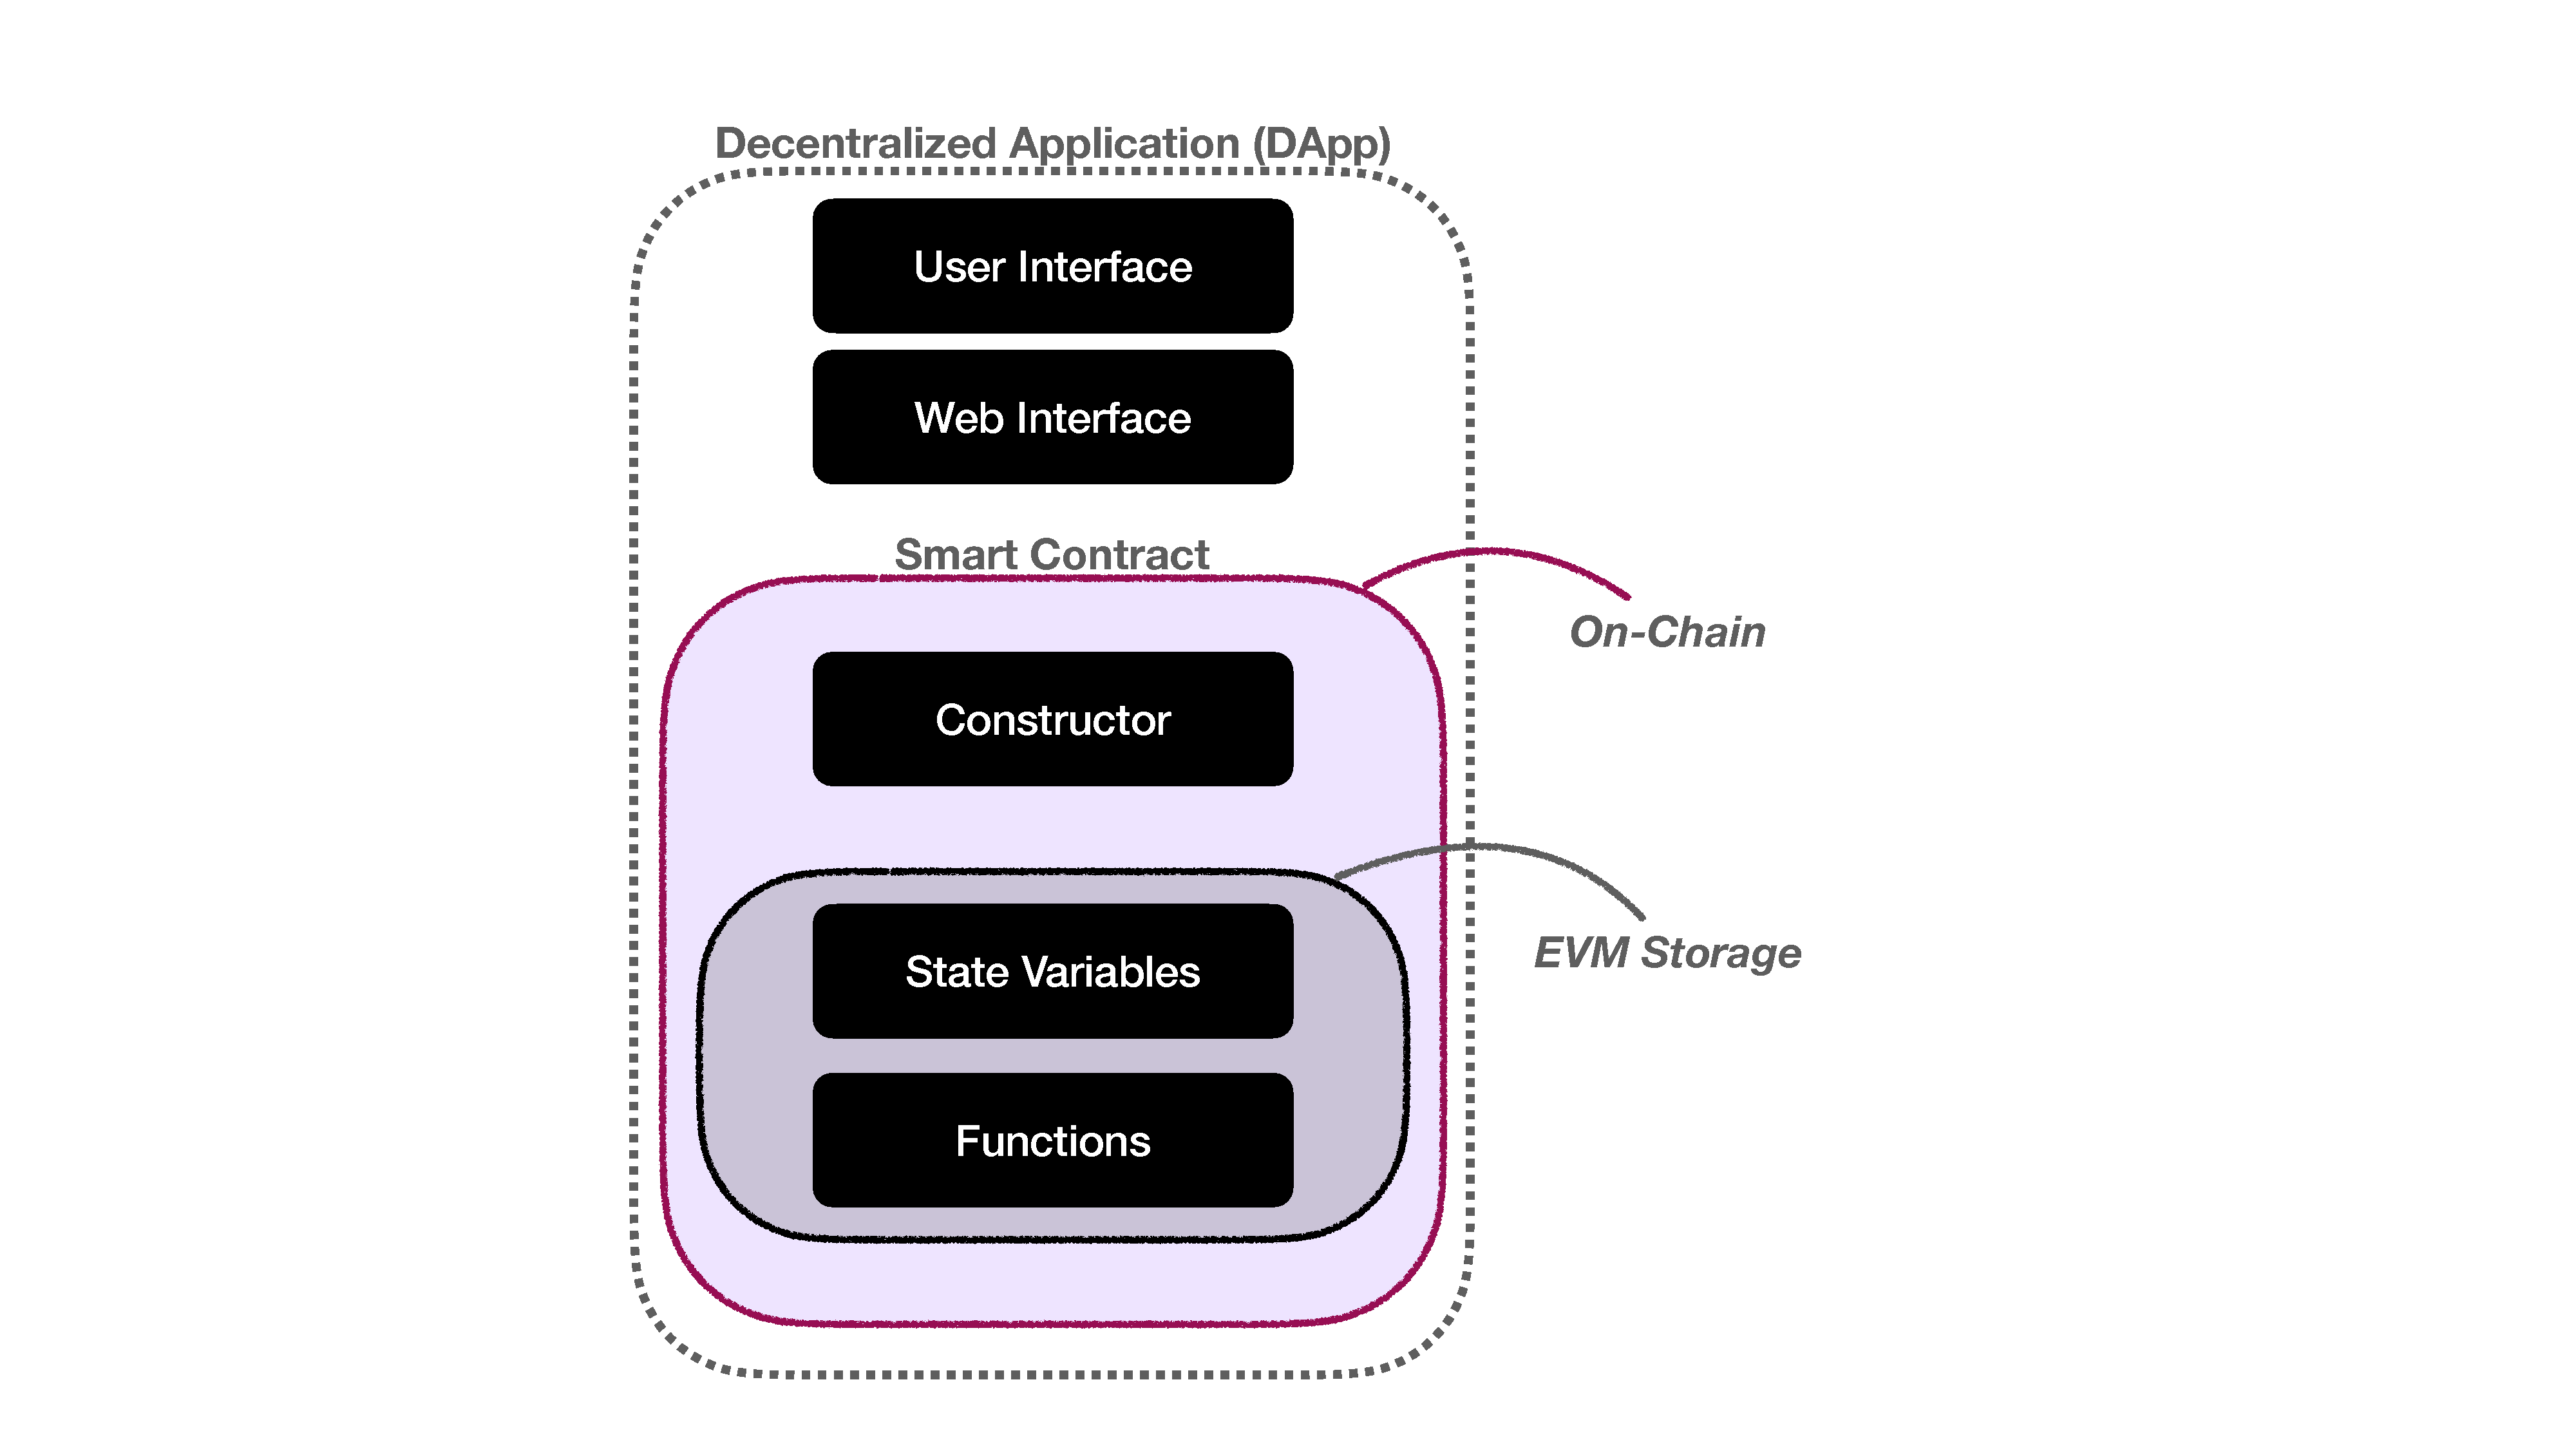
\includegraphics[width=0.4\textwidth]{figures/dapp.pdf}
%  \caption{Components of a decentralized application.\label{fig:dapp}}
% \end{figure}

%\paragraph{DApp vs. smart contract.} Figure~\ref{fig:dapp} shows the main components of a decentralized application (DApp). The core component is the smart contract (or simply contract), which is the set of functions and state stored on-chain. When first deployed, the smart contract also includes a constructor function which executes once and is then discarded (to be more precise, a copy of the constructor is stored in the record of transactions, called the calldata, but it is not retained in the EVM and can never be called again). While it is possible to interact directly with a smart contract by invoking its functions through Ethereum, generally users are provided an off-chain website with a user interface. Website actions are translated into calls to the Ethereum network through a set of tools (most prominently web3) in the web interface. 

% = = = = = = = = = = = = = = = = = = = = = = = = = = = = = = = = = = = = = = = = = =

\section{Classification of Upgrade Patterns} \label{sec:classification}

\paragraph{Updating vs. upgrading.} Software maintenance is part of software's lifecycle, and the process of changing the product after delivery. Often a distinction is drawn between software \textit{updates} and software \textit{upgrades}. An update modifies isolated portions of the software to fix bugs and vulnerabilities. An upgrade is generally a larger overhaul of the software with significant changes to features and capabilities. We only use the term upgrade and distinguish between retail (parameters and isolated code) and wholesale (entire application) changes to a smart contract. While upgrades to a smart contract's user interface (UI) can significantly change a user experience and expose new features, UIs are governed by traditional software maintenance. Our paper only considers the on-chain smart contract component, which is significantly more challenging to upgrade as it is on-chain and immutable under reasonable circumstances.

\begin{figure}[t]
  \centering
      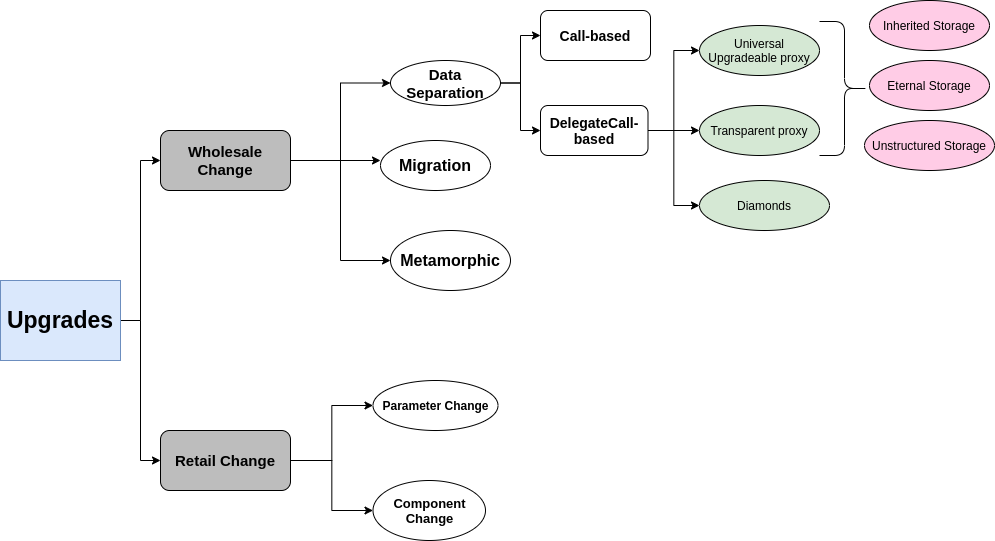
\includegraphics[width=0.8\textwidth]{figures/New_Classification.png}
  \caption{Classification of upgradeability patterns.\label{fig:class}}
 \end{figure}
 
A variety of upgradeability patterns have been proposed for smart contracts. Most leverage Ethereum-specific operations and memory layouts and are not applicable to other blockchain systems.

% Misc notes:
% We have some off-chain upgrades like what people did to force UNISwap using arbitrum as the L2 solution. It is an off-chain upgrade not an automated one.
% Does Factory patterns can be defined as upgradeability patterns? Like creating a new pool for Uniswap!


% JC: It seems the evaluation table will capture this. Plus are these pros/cons relative to each other or to other kinds of upgradeability (assuming the latter, it is hard to discuss until we have shown how they work). 
%The \textit{Pros and Cons} for retail changes methods are:
%\begin{itemize}
%  \item Pros
%  \begin{itemize}
%    \item Simple to implement
%    \item Easy to audit
%  \end{itemize}
%  \item Cons
%  \begin{itemize}
%    \item Cannot fix a bug
%    \item Cannot add/change Logic in Parameter Configuration
%    \item Cannot add new Logic in Tweak Strategy
%  \end{itemize}
%\end{itemize}

% = = =

\subsection{Parameter Configuration}
\label{sec:parameter}

We first categorize upgradeability patterns into two main classes: \textit{retail changes} and \textit{wholesale changes}. A pattern for retail change does not enable the replacement of the entire contract. Rather, a component of the contract is pre-determined (before the contract is deployed on Ethereum) to allow future upgrades, and the code is adjusted to allow these changes. 

The simplest upgrade pattern is to allow a system parameter, that is stored in a state variable, to be changed. This requires a \textit{setter function} to overwrite (or otherwise adjust) the variable, and access control over who can invoke the function. For example, in decentralized finance (DeFi), many services have parameters that control fees, interest rates, liquidation levels, \etc Adjustments to these parameters can initiate large changes in how the service is used (its `tokenomics'). A DeFi provider can retain control over these parameters, democratize control to a set of token holders (\eg stability fees in the stablecoin project MakerDao), or lock the parameters from anyone's control. In Section~\ref{sec:governance}, we dive deeper into the question who can upgrade a contract. 

% = = =

\subsection{Functional Component Change}
\label{sec:component}

While a parameter change allows an authorized user to overwrite memory, a functional component change addresses modifications to the code of a function (and thus, the logic of the contract). In the EVM, code cannot be modified once written and so new code must be deployed to a new contract, but can be arranged to be called from the original contract. 

One way to allow upgradable functions is deploying a helper contract that contains the code for the functions to be upgradeable. Users are given the address of the primary contract, and the address of this secondary contract is stored as a variable in the primary contract. Whenever this function is invoked at the primary contract, the primary contract is pre-programmed to forward the function call, using the opcode \texttt{Call}, to the address it has stored for the secondary contract. To modify the logic of the function, a new secondary contract is deployed at a new address, and an authorized set of individuals can then use a parameter change in the primary contract to update the address of the secondary contract.

The DeFi lending platform Compound~\footnote{\url{https://compound.finance}} uses this pattern for their interest rate models~\footnote{\url{https://github.com/compound-finance/compound-protocol/blob/v2.3/contracts/InterestRateModel.sol}} which are tailored specifically for each asset. The model for one asset can be changed without impacting the rest of the contract~\cite{openzeppelinPost}.

Upgradeable functional components need to be pre-determined before deploying the primary contract. Once the primary contract is deployed, it is not possible to add upgradeability to existing functions. It also cannot be directly used to add new functions to a contract. Finally, this pattern is most straightforward when the primary contract only uses the return value from the function to modify its own state. Thus, the function is either `pure' (relies only on the parameters to determine the output) or `view' (can read state from itself or other contracts, but cannot write state). If the function modifies the state of the primary contract, the primary contract must either expose its state variables to the secondary contract (by implementing setter functions), or it can run the function using \texttt{Delgatecall} if the secondary contract has no state of its own. 

This upgrade pattern suggests a way forward for wholesale changes to the entire contract: create a generic `proxy' contract that forwards all functions to a secondary contract. To work seamlessly, this requires some further engineering (sections~\ref{sec:callbased} and \ref{sec:delegatecall}).

% = = =

% \paragraph{Pluggable Modules}. In this pattern we have a core contract that have some immutable features and then new contracts generated by the main contract and each have some or all features of the main contract. This pattern is mostly used in wallets and DeFi services like DeFi saver and InstaDapp. Users can decide to add new features into their wallet. 


%We need upgradeability to fix a bug or adding a new feature. In the event of fixing a bug, the agent who is responsible for the upgrade need to be as quick as possible to address a security issue or bug and so there is no need to have consensus of the users of the Dapp to make change. But, in the latter case the agent must get the consensus of the Dapp users to change and add a new feature, so they do not need to be quick. This fact is another paradox in the upgradeability of smart contracts because these two different events are not distinguishable before occurring and so we cannot implement two different ways of upgrading a system (one for resolving bug, and one for adding feature). So, as a system designer, if decide to add upgradeability feature should select one of these as the main goal of adding upgradeability and design the system based on that.

% = = =

\subsection{Consensus Override}
\label{sec:hardfork}

The two previous patterns enable portions of a smart contract to be modified. The remaining patterns strive to allow an entire contract to be modified or, more simply, replaced. The first wholesale pattern is not a tenable solution to upgradeability as it as only been used rarely under extraordinary circumstances, but we include it for completeness. 

Immutability is enforced by the consensus of the blockchain network. If participating nodes (\eg miners) agreed to suspend immutability, they can in theory allow changes to a contract's logic and/or state. If agreement is not unanimous, the blockchain can be forked into two systems---one with the change and one without. In 2016, a significant security breach of a decentralized application called `the DAO' caused the Ethereum Foundation to propose overriding the immutability of this particular smart contract to reverse the impacts of attack. In the unusual circumstances of this case, it was possible to propose and deploy the fix before the stolen ETH could be extracted from the contract and circulated. Nodes with a philosophical objection to overriding immutability continued operating, without deploying the fix, under the name Ethereum Classic.
%Need to talk about L2 (Roll-ups) --> They can roll-back the chain state similar to the DAO fork (they can setup new desired rollup state and bridge regarding that).
%\textbf{Upgradeability is a Bug!}~\cite{Upg-Bug}.


% = = =

\subsection{Contract Migration}
\label{sec:migration}

The simplest wholesale upgrade pattern is to deploy a new version of the contract at a new address, and then inform users to use the new version---called a `social upgrade.' One example is Uniswap\footnote{\url{https://uniswap.org}}, which is on version 3 at the time of writing. Versions 1 and 2 are still operable at their original addresses. 

Contract migration does not require developers to instrument their contracts with any new logic to support upgradeability, as in many of the remaining patterns, which can ease auditability and gas costs for using the contract. However for most applications, there will be a need to transfer the data stored in the old contract to the new one. This is generally done in one of two ways. The first is to collect the state of the old contract off-chain and load it into the new contract (\eg via its constructor). If the old contract was instrumented with an ability to pause it, this can eliminate race-conditions that could otherwise be problematic during the data migration phase. The second method, specific to certain applications like tracking a user's balance of tokens, is to have the user initiate (and pay the gas) for a transfer of their balance to the new contract.
 
 % JC: do we *need* one or it is useful?
 %Also we need a \textit{Migrator} contract if we decided to outsource the data migration into the users.
 
 % = = =

\subsection{\texttt{CREATE2}-based Metamorphosis}
\label{sec:metamorphic}

Is it possible to do contract migration, but deploy the new contract to the \textit{same} address as the original contract, effectively overwriting it? If so, developers can dispense with the need for a social upgrade (but would still need to accomplish data migration). At first glance, this should not be possible on Ethereum, however a set of opcodes can be `abused' to allow it: specifically, the controversial\footnote{\href{https://www.reddit.com/r/ethereum/comments/lx32kv/expectations\_for\_backwardsincompatible\_changes/}{``Expectations for backwards-incompatible changes / removal of features that may come soon.'' V. Buterin, Reddit r/ethereum, Mar 2021.}} \texttt{SELFDESTRUCT} opcode and the 2019-deployed \texttt{CREATE2}. 

Consider a contract, called Factory, that has the bytecode of another contract, A, that Factory wants to deploy at A's own address. \texttt{CREATE2}, which supplements the original opcode \texttt{CREATE}, provides the ability for Factory to do this and know in advance what address will be assigned to contract A, invariant to when and how many other contracts that Factory might deploy.  The address is a structured hash of A's ``initialization'' bytecode, parameters passed to this code, the factory contract's address, and a salt value chosen by the factory contract.\footnote{Specifically: $\mathsf{addr} \leftarrow \mathcal{H}(\mathtt{0xff} \| \mathsf{factoryAddr} \| \mathsf{salt} \| \mathcal{H} (\mathsf{initBytecode} \| \mathsf{initBytecodeParams}))$} Most often, A's initialization bytecode contains a copy of A's actual code (``runtime'' bytecode) to be stored on the EVM, and the initialization code is prepended with a simple routine to copy the runtime code from the transaction data (calldata) into memory and return. Importantly, however, the initialization bytecode might not contain A's runtime bytecode at all, as long as it is able to fetch a copy of it from some location on the blockchain and load it into memory. In order for \texttt{CREATE2} to complete, the address must be empty, which means either (1) no contract has ever been deployed there, or (2) a contract was deployed but invoked \texttt{SELFDESTRUCT}.

%It is also common that A's initialization code will initialize some of A's storage variables (\eg the code specified in the constructor function in Solidity) using parameters passed into it. 

%The initialization bytecode passed to \texttt{CREATE2} will be recorded in the transaction call and then executed, but it is not stored in contract A. The expected result of executing the initialization bytecode is that contract A's runtime bytecode will be deployed at the determined address. 

Assume the developer wants to deploy contract A using metamorphosis and later update it to contract B.\footnote{\href{https://medium.com/@0age/the-promise-and-the-peril-of-metamorphic-contracts-9eb8b8413c5e}{``The Promise and the Peril of Metamorphic Contracts.'' 0age, Medium, Feb 2019.}} The developer first deploys a factory contract with a function that accepts A's (runtime) bytecode as a parameter (which includes the ability to self destruct). The factory then deploys A at an arbitrary address and stores the address in a variable called codeLocation. The factory then deploys a simple `transient' contract using \texttt{CREATE2} at address T. This contract performs a callback to the factory contract, asks for factory.codeLocation, and copies the code it finds there into its own storage for its runtime bytecode and returns. As a consequence, A's bytecode is now deployed at address T. 

To upgrade to contract B, the developer calls \texttt{SELFDESTRUCT} on A. Mechanically, the consequences of \texttt{SELFDESTRUCT} on the EVM are only realized at the end of the transaction. In a followup transaction, the developer calls the factory with contract B's bytecode. The factory executes the same way placing a pointer to B in factory.codeLocation. Importantly, it generates the same address T when it invokes \texttt{CREATE2} since the `transient' contract is identical to what it was the first time---this contract does not contain contract A or B's runtime code, it just contains abstract instructions on how to load code. The result is contract B's runtime bytecode being deployed at address T where contact A was. 
 
% JC: Not important enough to keep:
%One limitation of this pattern is that Contract A and B cannot make use of a constructor, as the constructor is utilized by the transient contract. However contract A and B can implement a constructor-esque function that the factory invokes after \texttt{CREATE2} and  modifiers in the contract enforce it is only executable once. The only tangible difference is that its code will be stored as part of its runtime bytecode, whereas real constructor code is executed once and discarded (it is still recorded in the calldata of the transaction that creates the contract). 

As it is concerning that a contract's code could completely change, we note that metamorphic upgrades can be ruled out for any contract where either: it was not created with \texttt{CREATE2}, it does not implement \texttt{SELFDESTRUCT}, and/or its constructor is not able to dynamically modify its runtime bytecode. 

%This type of upgradeability is relevant to \textit{Create2} opcode which is proposed by Vitalik Buterin in 2018-04-20 as EIP-1014. To create a new contract in Ethereum blockchain we have 2 different opcodes; Create and Create2. The main difference between these two is the address of the contract that is going to be deployed. In Create opcode the address depends on the address and nonce of the creator. Nonce is a number regarding to the account and is like a counter to the number of transactions sent by that account (for contract account nonce is the number of contracts that are deployed by that contract). The problem of using Create opcode for contract deployment is that we cannot have a way to calculate the address of deployed contract because it depends on the nonce of the sender. Create2 opcode solve this problem because the address of the deployed contract just depends on the address of deployer and the \textit{Bytecode} of the contract to be deployed (and also a salt number which the deployer should specify each time). So we can hardcode the address of the deployed contract before deployment if we uses Create2.


%$\mathsf{addr} \leftarrow \mathcal{H}(\mathtt{0xff} \| \mathsf{facoryAddr} \| \mathsf{salt} \| \mathcal{H} (\mathsf{bytecode} \| \mathsf{owner} \| \mathsf{constructorParams}))$


%The other important property of Create2 opcode is that it uses \textit{init code} as the bytecode to calculate the address for deployment. The init bytecode is the bytecode which the creator will send to Ethereum blockchain and it is different from the \textit{Runtime Bytecode}. In fact, the EVM will execute constructor before deployment of the contract and then change the bytecode to the runtime code so the main difference between init bytecode and runtime bytecode is the constructor.

%In Metamorphic upgrade pattern, we abuse the Create2 opcode and take advantage of the difference between init bytecode and runtime bytecode to redeploy a contract with a new logic in the same address. To describe the process completely we should describe the Metamorphic Contract Factory a bit. This factory contract clones the implementation contract in its constructor and deploy the new bytecode on the previous address. The key idea is that the bytecode that we are going to deploy has a constructor that changes the bytecode to what we want to be deployed. So the init bytecode is the same as the previous deployment but the runtime bytecode is the new bytecode that we want to deploy.

%There is a critical point here. Before deploying a new contract on that exact address, the previous contract should be self destructed. Note that self destruct will wipe out the storage of the contract. So, in metamorphic upgradeability pattern we will lose the data and so we should migrate the data manually after deployment. In fact this type of upgradeability pattern is good for stateless contracts or contracts that has a limited storage variables (e.g. Beacon contract). The greatest risk to this type of upgradeability pattern is that there is a huge debate on the Ethereum community to remove the self-destruct opcode and without the self-destruct opcode the pattern is broken. 

% JC: will compare after discussion proxy patterns
%In comparison to the proxy patterns, metamorphic pattern is more gas efficient because we don't need to have any checks like what we had in transparent proxy or also we don't have the delegate call process. Similar to proxy contract, after upgrade the address of new version is not changed but we need to migrate the old data to the newer version. Also in metamorphic pattern there is downtime to the system because we should firs self-destruct the previous contract and the process of self-destructing occurs at the end of the transaction. So, we should first self-destruct the old version in a transaction and then redeploy the contract in another transaction and there is a downtime between these 2 transactions.


% = = =

\subsection{\texttt{CALL}-based Data Separation}
\label{sec:callbased}

To avoid migrating the stored data from an old contract to an upgraded contract, a contract could instead store all of its data in an external ``storage'' contract. In this pattern, calls are made to a ``logic'' contract which implements the function (or reverts if the function is not defined). Whenever the logic contract needs to read or write data, it will call the storage contract using setter/getter (aka accessor/mutator) functions. An upgrade consists of (1) deploying a new logic contract, (2) pausing the storage contract, (3) granting the new logic contract access to the storage contract, (4) revoking access from the old contract, and (5) unpausing the storage contract. 

An important consideration is that the layout of the storage contract cannot be changed after deployment (\eg we cannot add a new state variable). This can be side-stepped to some extent by implemented a mapping (key-value pair) for each primitive data type. For example, a new uint state variable can be a new entry in the mapping for uints. This is called the Eternal Storage pattern (ERC930). It however requires that every data type be known in advance, and is challenging to use with complex types (\eg structs and mappings themselves).

A variant of this pattern can introduce a third kind of contract, called a proxy contract, to address the social upgrade problem. In this variant, users permanently use the address of the proxy contract and always make function calls to it. The proxy contract stores a pointer (that can be updated) to the most current logic contract, and asks the logic contract to run the function using \texttt{CALL}. Unlike the functional component pattern (Section~\ref{sec:component}), the proxy will catch and forward \textit{any} function (including new functions deployed in updated logic contracts) using its fallback function.  With or without proxies, this pattern is very powerful, but instrumenting a contract to use it requires deep-seated changes to the contract code. As our measurements will show, it has fallen out of favour for the cleaner \texttt{DELEGATECALL}-based pattern (Section~\ref{sec:delegatecall}) that addresses the same issues with simpler instrumentation. 

% JC: already covered by contract migration :
%In this type of upgrade the address of the contract will be changed after upgrade so we need to aware our users about the change and interacting with the new version. Also it may break the compatibility of the ecosystem. In case of upgrade all smart contracts and Dapps that are interacting with the upgraded smart contract must change the address which they pointed to in order to interact with our contract. It may leads into a disaster if other contracts that are interacting with our contract do not have a way to change the address. We should also make other off-chain services (e.g. exchanges) aware of the change to start using the new version of your contract. In Call-based pattern we should have a way to stop previous version during/after upgrade because both of them are shared the same storage contract. 

% JC: this is covered I think
%There are three main ways to implement upgrades using data separation pattern. The easiest way is to change the ownership of storage contract into new upgraded logic contract and then \textit{Pause} the old contract using \textit{Circuit Breaker} pattern or set its pointer to 0x0 address. The other solution is to forward the calls receive by the old contract into the new logic contract. The last option is to set a registry contract that just keeps the address of latest version of the logic contract and call into it.

% JC:  Save evaluation for the table
% Using Calls-based pattern we eliminate the process of data migration from the old contract to the newer version and it is easy to understand this type of upgradeability pattern. But it is hard for developers to deal with this pattern when their logic contract needs complex data structures such as mapping or structures. Also the developers should change their code a lot if they decide to use this upgradeability pattern in their non-upgradeable code. 

% = = =

\subsection{\texttt{DELEGATECALL}-based Data Separation}
\label{sec:delegatecall}
%In this pattern, a typical function call is chained through three contracts. The call is always made to the same contract, called the proxy contract, that is deployed permanently at a given address. The proxy contract stores a pointer to a second contract, called the logic contract, and implements only a few basic functions (\eg for updating the pointer). Any function (with any other function name) that is invoked is caught by the contract's fallback function and forwarded with the parameters, using \texttt{CALL}, to the logic contract. 

%function () payable public {
%        address target = logic_contract;
%        assembly {
%            let ptr := mload(0x40)
%            calldatacopy(ptr, 0, calldatasize)
%            let result := delegatecall(gas, target, ptr, calldatasize, 0, 0)
%            let size := returndatasize
%            returndatacopy(ptr, 0, size)
%            switch result
%            case 0 { revert(ptr, size) }
%            case 1 { return(ptr, size) }
%        }

This pattern is a variant on the idea of chaining each function call through a sequence of three contracts: proxy, logic, and storage. The first modification is reversing the sequence of the logic and storage contracts: a function call is handled by the proxy which forwards it to the storage contract (instead of the logic contract). The storage contract then forwards it to the logic contract using \texttt{DELEGATECALL} which fetches the code of the function from the logic contract but (unlike \texttt{CALL}) runs it in the context of the contract making the call---\ie the storage contract. When upgrading, a new logic contract is deployed, the proxy still points to the same storage contract, and the storage contract points to the new logic contract. Since the proxy and storage contracts interact directly and are both permanent, the functionality of both can be combined into a single contract. It is common for developers to call this the `proxy contract,' despite it being a combination of a proxy and a storage contract. 

This pattern is generally cleaner than using the previous \texttt{CALL}-based pattern because the logic contract does not need any instrumentation added to it. It is an exact copy of what the contract would look like if the upgrade pattern was not being used at all. However this does not mean the pattern in a turn-key solution. Each new logic contract needs to be programmed to respect the existing memory layout of the storage contract, which has evolved over the use of all the previous logic contracts. The logic contract also needs to be aware of any functions implemented by the storage contract itself---if the same function exists in both the storage contract and the logic contract (called a function clash), the storage function will take precedence.

% JC: upgradeTo in old logic contract, delegateCall to it
% JC: add access control everywhere

The main issue with function clashes is that the proxy contract needs, at the very least, to provide an admin (or set of authorized parties) the ability to change the address of the logic contract it delegates to. This can be addressed in four main ways:

\begin{enumerate}

%If this is captured by a function deployed in the proxy contract,  say \texttt{setLogicContract(addr a)}, then any other function signature will be caught by the proxy's fallback function which will \texttt{DELEGATECALL} it to the current logic contract. 

\item Developers are diligent that no function signature in the logic contract is equal to the signature of this function in the proxy contract (note that signatures incorporate a truncated hash of the function name, along with the parameters types, so collisions are possible). 

\item As found in the \emph{universal upgradeable proxy standard (UUPS)} (EIP-1822): implement the upgrade function in the logic contract, which will run in the context of the proxy contract. Its exact function signature must be hardcoded into the proxy contract. Every logic contract update must include it or further updates are impossible.

\item As found in the \textit{beacon proxy} pattern (EIP-1967): deploy another contract, called the beacon contract, to hold the address of the logic contract and implement the setter function for it. The proxy contract will get the logic contract address from the beacon every time it does a \texttt{DELEGATECALL}. The admin calls the beacon contract to upgrade the logic contract, while normal users call the proxy contract to use the DApp. 

\item As found in the \textit{transparent proxy} pattern (EIP-1538): inspect who is calling the proxy contract (using \texttt{msg.sender()})---if it is the admin, the proxy contract catches the function call and if it is anyone else, it is passed to the proxy's fallback function for delegation to the logic contract. 

\end{enumerate}

%For some decentralized applications, many copies of the same contract are made. For example, in an on-chain wallet solution, every user might be given their own wallet contract at their own address with only their data stored in it. Consider making such an application upgradable using UUPS. If there are $n$ users, each user gets its own proxy contract (thus $n$ proxy contracts). However the logic contract can be shared across all users. In the \textit{Beacon Proxy} pattern (EIP-1538), a common ``beacon'' contract is hard-coded into all proxy contracts and allows them to obtain the latest logic contract. 

A drawback of the entire \texttt{DELEGATECALL}-based pattern is that logic contracts need to be aware of the storage layout of the proxy contract. In a stand-alone contract, the compiler (\eg Solidity) will allocate state variables to storage locations, and using \texttt{DELEGATECALL} does not change that, however new logic contracts need to allocate the same variables in the same order as the old contract, even if the variables are not used anymore. This can be made easier with object-oriented patterns: each new logic contract extends the old contract (inheritance-based storage). Other options include mappings for each variable type (eternal storage) or hashing into unique memory slots (unstructured storage). The \textit{Diamond Storage} pattern (EIP-2535) breaks the logic contract into smaller clusters of one or a few functions that can be updated independently, and each can request one or more storage slots in a storage space managed by the proxy contract itself. 

% JC: Diamond sharded -> large contracts



%\paragraph{Beacon Proxy}. 



%Next consider techniques for ensuring new logic contracts respect the storage layout of the storage contract. 
%\begin{itemize}
%\item \textbf{Inherited Storage}. 
%In this method the proxy and all logic contracts are inherited from a storage contract that contains storage variables. If we decided to upgrade the contract, we should be sure that the new implementation contract is inherited from the storage contract. Using this method we are confident that the proxy and logic contracts are using the same storage layout and storage clashes will be mitigated.
%Also if after deployment we need to add new storage variables, we should just deploy a new storage contract that inherited from the previous storage contract and add the new variables to it. We should be sure that the future implementation contracts will inherit the latest storage contract. This adds-on to the inherited storage contract is called append-only pattern.
%This method is not efficient because of variables that declared but not used in some logic contracts. On the other hand, each logic contract is coupled with a storage contract and it is hard to take care of this track. Also we should take care of upgrading the system each time to be sure that the new implementation contract is inherited from the latest version of storage contract.
%
%\item \textbf{Eternal Storage}. 
%As described before in Eternal storage, we defined mappings for all variable types that we need to use in our logic smart contract. For storing mapping variables EVM selects random slots on the storage based on the variable's name so we can mitigate the clashes using this randomness.
%The main problem of this type is that the logic contract and all other contracts that are using the storage must use the mapping structure to access the storage variables and use complex syntax whenever they want to access a variable. This also results in the gas usage inefficiency because we need to call and update a mapping each time we need to change a variable.  
%
%
%\item \textbf{Unstructured Storage}. 
%The other way of mitigating the storage clashes is to assign some randomly selected slots to critical variables like address of logic contract. For instance, openzeppelin uses hash of "org.zeppelinos.proxy.implementation" to store the address of the logic contract in this slot.
%The downside of this approach is that we need getter and setter function for each variable. We also can use unstructured storage for simple variables and not for mapping and structures. EIP-1967 proposed to assign specific storage slots for address variable inside the proxy contract to store the address of the implementation contract inside the proxy. The proposed slot is 0x360894a13ba1a3210667c828492db98dca3e2076cc3735a920a3ca505d382bbc which is calculated from this equation
%bytes32(uint256(keccak256(eip1967.proxy.implementation)) - 1)). 
%%% Add exact gas cost from the image
%
%\end{itemize}

%\paragraph{Diamonds}
%The \textit{Diamond Standard} pattern (EIP-2535) is proposed on 2020-02-22 and suggested using multi implementation contracts with a single proxy contract. In the proxy there is a access control structure in which there is a mapping between each implementation contract's address and the function signatures that are implemented inside that specific implementation contract. Using this method we can have a separate implementation contract for each functionality of the Dapp. It will help to make the contracts more modularize. Also we can just update one functionality in each upgrade event. It also helps with the situation that the contract code size exceeds the limitation (24KB) by splitting it into a number of implementation contracts.
%
%The drawback of using Diamonds is adding more complexity to the system because using different implementation contracts will increase the chance of storage clashes and error in handling the shared storage between them.




\subsection{Evaluation Framework}
% !TEX root = ../main.tex

\begin{table}[t!]
    \centering
    
        \begin{tabular}{lllllllllllllll}
    
    &
    \headrow{Can replace entire logic} &
    
    \headrow{can replace pre-specified part of logic} & 


    \headrow{Can replace entire state} &
    
    \headrow{can change pre-specified state variables} &
    
    \headrow{No need to deploy a new contract} &

    \headrow{No need to migrate state from old contract} &

    \headrow{No need to separate State and Logic} &

    \headrow{Function Selector Clashes Risk} &

    \headrow{Storage Clashes Risk} & 

    \headrow{No indirection} & 


    \headrow{User endpoint address not changed} &
    

    \headrow{Downtime in upgrade events} &

    \headrow{No need to change code to add the upgrade pattern} &

    \headrow{Need to change a state variable} 
    
    
    \\
    
    \hline
 
    
        \multicolumn{1}{c|}{Parameter change}	& \multicolumn{1}{c|}{}  & \multicolumn{1}{c|}{} &  \multicolumn{1}{c|}{} & \multicolumn{1}{c|}{\checkmark} & \multicolumn{1}{c|}{\checkmark} & \multicolumn{1}{c|}{\checkmark} &  \multicolumn{1}{c|}{\checkmark} &  \multicolumn{1}{c|}{} & \multicolumn{1}{c|}{} & \multicolumn{1}{c|}{\checkmark} & \multicolumn{1}{c|}{\checkmark} & \multicolumn{1}{c|}{} &\multicolumn{1}{c|}{\checkmark} & \multicolumn{1}{c}{\checkmark}\\
    
        \hline
  
        \multicolumn{1}{c|}{Component Change}	& \multicolumn{1}{c|}{}  & \multicolumn{1}{c|}{\checkmark} &  \multicolumn{1}{c|}{} & \multicolumn{1}{c|}{} & \multicolumn{1}{c|}{} & \multicolumn{1}{c|}{\checkmark} &  \multicolumn{1}{c|}{\checkmark} &  \multicolumn{1}{c|}{} &  \multicolumn{1}{c|}{} &  \multicolumn{1}{c|}{\XBox} & \multicolumn{1}{c|}{\checkmark} & \multicolumn{1}{c|}{} & \multicolumn{1}{c|}{\XBox} &  \multicolumn{1}{c}{\checkmark}\\
        

        \hline

        \makecell{Migration}	& \multicolumn{1}{|c|}{\checkmark}  & \multicolumn{1}{c|}{} &  \multicolumn{1}{c|}{\checkmark} & \multicolumn{1}{c|}{} & \multicolumn{1}{c|}{} & \multicolumn{1}{c|}{} &  \multicolumn{1}{c|}{\checkmark} &  \multicolumn{1}{c|}{} &  \multicolumn{1}{c|}{} &  \multicolumn{1}{c|}{\checkmark} & \multicolumn{1}{c|}{} & \multicolumn{1}{c|}{} & \multicolumn{1}{c|}{\checkmark} &  \multicolumn{1}{c}{}\\
    
         \hline


        \makecell{Call-based}	& \multicolumn{1}{|c|}{\checkmark}  & \multicolumn{1}{c|}{} &  \multicolumn{1}{c|}{} & \multicolumn{1}{c|}{} & \multicolumn{1}{c|}{} & \multicolumn{1}{c|}{\checkmark} &  \multicolumn{1}{c|}{} &  \multicolumn{1}{c|}{} &  \multicolumn{1}{c|}{} &  \multicolumn{1}{c|}{} & \multicolumn{1}{c|}{} & \multicolumn{1}{c|}{} & \multicolumn{1}{c|}{} & \multicolumn{1}{c}{\checkmark}\\
    
        \hline


        \makecell{DelegateCall-based}	& \multicolumn{1}{|c|}{\checkmark}  & \multicolumn{1}{c|}{} &  \multicolumn{1}{c|}{} & \multicolumn{1}{c|}{} & \multicolumn{1}{c|}{} & \multicolumn{1}{c|}{\checkmark} &  \multicolumn{1}{c|}{} &  \multicolumn{1}{c|}{\checkmark} & \multicolumn{1}{c|}{\checkmark}&  \multicolumn{1}{c|}{} & \multicolumn{1}{c|}{\checkmark} & \multicolumn{1}{c|}{} & \multicolumn{1}{c|}{\XBox} & \multicolumn{1}{c}{\checkmark}\\

        \hline

        \makecell{Diamonds}	& \multicolumn{1}{|c|}{\checkmark}  & \multicolumn{1}{c|}{} &  \multicolumn{1}{c|}{} & \multicolumn{1}{c|}{} & \multicolumn{1}{c|}{} & \multicolumn{1}{c|}{\checkmark} &  \multicolumn{1}{c|}{} &  \multicolumn{1}{c|}{\checkmark} & \multicolumn{1}{c|}{\checkmark\checkmark}&  \multicolumn{1}{c|}{} & \multicolumn{1}{c|}{\checkmark} & \multicolumn{1}{c|}{} & \multicolumn{1}{c|}{\XBox} & \multicolumn{1}{c}{\checkmark}\\
        
        
         \hline

        \makecell{Metamorphic}	& \multicolumn{1}{|c|}{\checkmark}  & \multicolumn{1}{c|}{} &  \multicolumn{1}{c|}{\checkmark} & \multicolumn{1}{c|}{} & \multicolumn{1}{c|}{} & \multicolumn{1}{c|}{} &  \multicolumn{1}{c|}{\checkmark} &  \multicolumn{1}{c|}{} & \multicolumn{1}{c|}{}&  \multicolumn{1}{c|}{\checkmark} & \multicolumn{1}{c|}{\checkmark} & \multicolumn{1}{c|}{\checkmark} & \multicolumn{1}{c|}{\checkmark} &  \multicolumn{1}{c}{}\\
        
        
         \hline
        
        
        \end{tabular}
        \captionsetup[tabular]{singlelinecheck=off}
        \caption{Evaluation}
       
    
    \end{table}
    \footnotetext[1]{Design of system in which a parameter can change the logic is hard}

Table~\ref{tab:eval} summarizes the pros and cons of each upgradeability pattern, omitting consensus override as it is only used in emergencies. Further detail and some take-aways from the evaluation are in Appendix~\ref{app:eval} and~\ref{app:eval2}. % The details of the evaluation are provided in the full version of this paper.\footnote{To be archived. Can be provided anonymously though program chairs.}




 %%%%%%%%%%%%%%%%%%%%%%%%%%%%%%%%%%%%%%%%%%%%%%%%%%%%%%%%%%%%%%%%%%%%%%%%%%%%%%%%%%%%%%%%%%%%%%%%%%%%%%%%%%%%%%%%%%%%%%%%%%%%%%%%%%%%%%
 %%%%%%%%%%%%%%%%%%%%%%%%%%%%%%%%%%%%%%%%%%%%%%%%%%%%%%%%%%%%%%%%%%%%%


 \section{Finding Upgradeable Contracts} 
 \label{sec:proxyFinding}
 
We now design a series of measurement studies to shed light on the prevalence of the various upgrade patterns. We exclude retail changes from our measurements, because variable changes and external function calls are too commonplace to distinguish. We focus on wholesale patterns, and devote the most effort to finding contracts using the \texttt{DELEGATECALL}-based data separation pattern (Section~\ref{sec:delegatecall}) as these are the most widely used and there are various sub-types (UUPS, beacon, \etc). The other types of wholesale patterns are: 
\begin{itemize}
\item \textbf{Consensus override:} Only 1 occurrence to date (the DAO attack~\cite{dhillon2017dao}).
\item \textbf{Contract migration:} Not detectable in code; relies on social communication of the new address.
\item \textbf{\texttt{CREATE2}-based metamorphosis.} Already measured by Frowis and Bohme~\cite{frowisnot} in a broader study of all uses of \texttt{CREATE2}. They found 41 contracts between March 2019 and July 2021 that upgraded using this pattern.
\item \textbf{\texttt{CALL}-based data separation.} We conducted a quick study of 93K contracts with disclosed source code~\cite{smart_contract_sanctuary}. We identified the Eternal Storage pattern using regular expressions and found 140 instances, the newest having been deployed over 3.5 years old. We conclude this pattern is too uncommon today to pursue a deeper bytecode-based on-chain measurement.  
\end{itemize}



% This section aims to shed light on the state of upgradeable smart contracts on the Ethereum blockchain. Between all the different patterns described in previous sections, we focused on finding the \textit{Delegate-call} based upgradeable contracts because it is the most widely used pattern for smart contract upgradeability at the time of writing this paper. The number of Ethereum Improvement Proposals (EIPs) and standards proposed for standardizing this pattern (e.g., EIP-1967, EIP-1822, EIP-2535, etc.) confirms this point. In the further parts of this section, we focus on describing the methodology used for finding upgradeable contracts in Ethereum blockchain, which use \textit{Delegatecall-based} patterns and show the results. 
%Here I have the reason why we chose delegate call based patterns:

%There is no general way to detect \textit{Retail Change} patterns in large-scale, in which one or multiple state variables can be changed inside the contract by admin of the contract, because there is no general way to distinct between a changeable state variable inside a contract that can be updated and non-critical one. It really depends on the business logic of the smart contract.

%\textit{Wholesale change} approaches consist of \textit{Call-based}, \textit{Delegatecall-based} and \textit{Metamorphic} patterns. The Call-based pattern is an old fashion way of adding upgradeability to a system. This type is not widely used nowadays. On the other hand, \textit{Delegate-call}  pattern is the most-used pattern in ethereum contracts and this is why we focused on this pattern in our research. \textit{Metamorphic} pattern is very new and not well-tested yet. Also it has limitations such as the state of the contract should wiped out before upgrade each time because of need of self-destruction. Also there are some risks to this pattern. For instance there are discussions in Ethereum community about removing \textit{Selfdesctruct} opcode from EVM~\cite{selfDestruct}. 

%In the above paragraph we claimed that the \textit{Call-based} pattern is not widely used these days. To prove this claim we perform an analysis on 93,000 verified smart contracts in smart contract sanctuary database~\cite{smart_contract_sanctuary} which gathers all verified smart contracts from \textit{Etherscan} blockchain explorer. As mentioned in previous sections \textit{Call-based} patterns consist of a logic contract and storage contract. The storage contract should define all storage variables needed for the system and must have getters and setters for these variables. Storage contract is the part that is not changing in upgrade events. So the developers should be sure that all state variables that are needed are defined in the deployment time or using tricks and patterns that give the developers ability to add new state variables after deployment. \textit{Eternal Storage} pattern is using a key-value based structure for the storage contract by using \textit{mappings} for defining all variables which gives the developers ability to add new variables after deployment. This is the reason that why Eternal Storage is widely used as the storage contract in \textit{Call-based} patterns. In this analysis, we try to find contracts that uses eternal storage structure in their logic using Regular Expression analysis. \emph{470} contract are found that uses eternal storage patterns and then we filtered them to find contracts that uses eternal storage structure and only contains getter and setter functions and not any other logics (the reason is described in the previous sections). After filtering we come up with \emph{170} unique eternal storage contracts that are used as storage contract of upgradeable Dapps. Checking the time of deployment of these contracts show that the latest one was deployed on July 2018 which show that this pattern is not widely used anymore these days (the reasons are discussed in the evaluation section).


\subsection{Methodology} 

\begin{figure}[t!]
  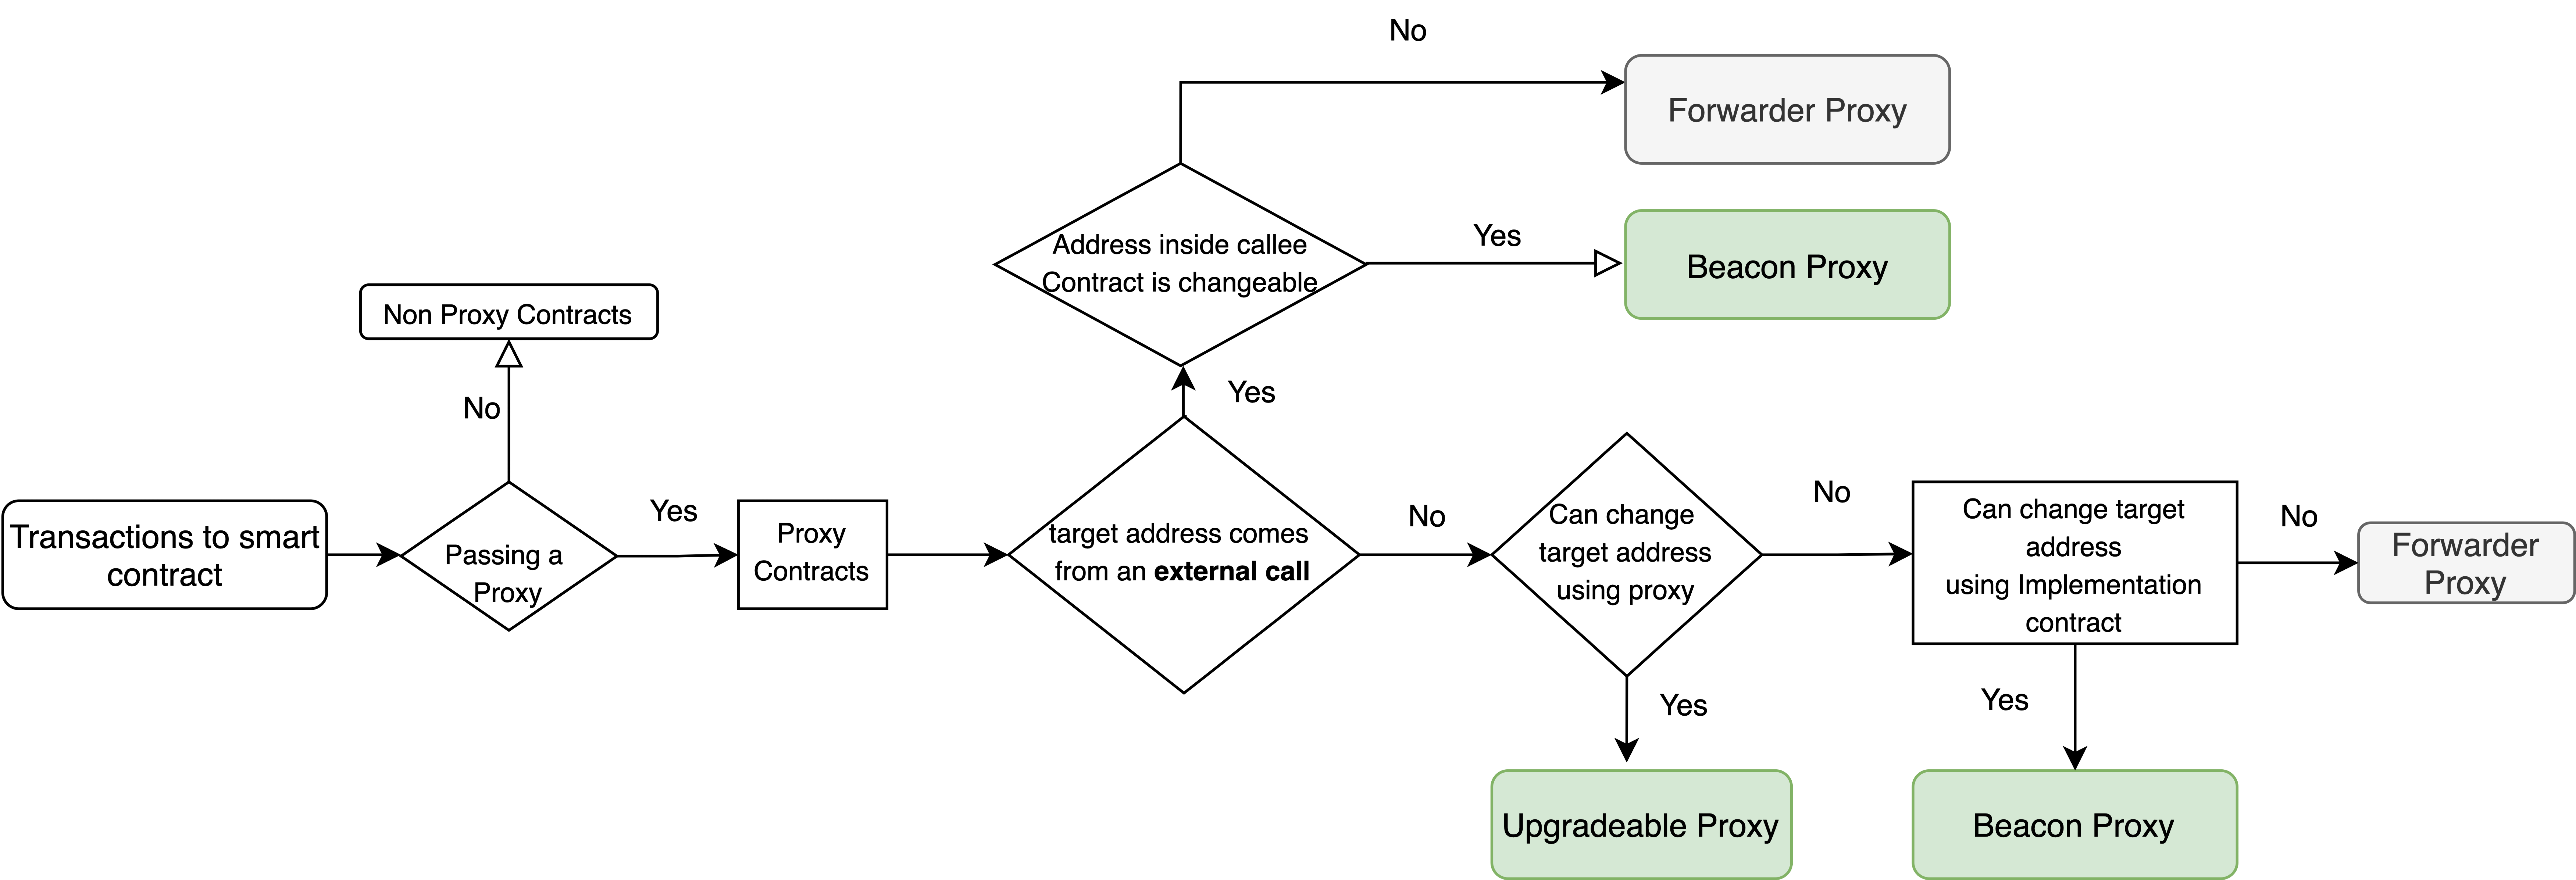
\includegraphics[width=1\textwidth]{New-method.png}\label{flowchart}
  \caption{Flowchart for distinguishing upgradeable contracts (green) from forwarders, and for determining the upgradability pattern type.}
\end{figure}

% % %

\paragraph{Finding proxies.} While not every use of a proxy contract is for upgradeability (\eg minimal proxies~\cite{minimalProxy}, \texttt{DELEGATECALL} forwarders~\cite{delegatecallForwarders}, \etc), all \texttt{DELEGATECALL}-based upgradeability variants have the functionality of a proxy. We therefore start by measuring the number of contracts with a proxy component, and then filter out the \textit{Forwarders} which do not enable upgradeability. To identify proxies, we examine every \texttt{DELEGATECALL} action and see if it was proceeded by a call with an identical function selector to the contract making the \texttt{DELEGATECALL} action, which indicates   the contract does not implement this function and instead caught it in its fallback function, and is now forwarding it to another contract at, what we will call, the \textit{target address}. We used an Ethereum full archival node\footnote{\url{https://archivenode.io/}} and replayed each transaction in a block to obtain Parity VM transaction traces. \texttt{DELEGATECALL} is one \texttt{callType} of an \texttt{action} within a trace. Specifically, if the data of two consecutive actions of a transaction are equal and a \texttt{DELEGATECALL} is in the second action, it shows that the transaction passes the fallback function (if any other function in the contract is called, other than fallback, then the first four bytes of the data will be changed). The \texttt{DELEGATECALL} indicates the fallback transferred the whole data to the target address without altering it, which means the contract implements a proxy.

\paragraph{Distinguishing forwarders and upgradability patterns.} In an upgradeable contract, the target address for the \texttt{DELEGATECALL} must be modifiable. If it is fixed, we tag it as a forwarder. We define five common patterns for determining the target address cannot be changed:

\begin{enumerate}
  \item The target address is hardcoded in the contract.
  \item The target address is saved in a constant variable type.
  \item The target address is saved in an immutable variable type and the deployer sets it in a constructor function.
  \item The target address is defined as an unchangeable storage variable.
  \item The proxy contract grabs the target address by calling another contract but there is no way the callee contract can change this address.
\end{enumerate}

In the first three situations, the target address will be appeared in the runtime bytecode of the contract. For every proxy-based \texttt{DELEGATECALL}, we obtain the target address from the transaction's \texttt{to address}, and we obtain the caller's bytecode by invoking \texttt{eth\_getCode} on the full node. If we find the target address in the bytecode, we mark it as a forwarder. 

In the fourth case, we find where the target address is stored by the contract by decompiling the contract, with \textit{Panoramix}\footnote{\url{https://github.com/palkeo/panoramix}}, locating the line of code in the fallback function that makes the \texttt{DELEGATECALL}, and marking the storage slot for the target address. We parse the code and check if an assignment to that slot happens in any function in the contract---this is non-trivial and we refer the interested reader to Appendix~\ref{app:assignment} for the full details. If any assignment is found, we should be sure that the other variable assigned to the target address variable comes from the input of that function. If these conditions are satisfied, there is a function inside the contract that can change the target address and we mark the proxy as an upgradeable proxy contract. 

Recall in the Universal Upgradeable Proxy Standard (UUPS) pattern, the logic contract implements a function to update the target address that is run in the proxy contract's context using \texttt{DELEGATECALL}. This is a subcase of the fourth case, where we checked the logic contract instead of the proxy contract. If we determine the logic contract can assign values to the logic contract in any function, we tag it as UUPS.

In the fifth case, we rewind the transaction trace from the proxy-based \texttt{DELEGATECALL} and look for the target address being returned to the proxy contract in another action. If we find it being returned by a contract, we apply the methodology from the fourth case to this contract. If the target address is modifiable, we mark it as using the Beacon proxy upgradability pattern. All contracts that remain after performing all of the checks above are marked as forwarders. 

\subsection{Results}

\begin{table}[t]
\centering
\begin{tabular}{|l|r|}
\hline
Proxy Contracts (Total) & 1,427,215  \\ \hline 
Proxy Contracts (Filtered) & 13,088  \\ \hline 
Regular Upgradeable Contracts & 7,470  \\ \hline
UUPS & 403  \\ \hline
Beacon & 352  \\ \hline
\end{tabular}
\caption{\label{tab:updata} Results of each \texttt{DELEGATECALL}-based upgrade pattern for the time-period {Sep-05-2020} to {Jul-20-2021} (2,064,595 blocks).}
\vspace{-10pt}
\end{table}

Our measurements cover block number \texttt{10800000} to \texttt{12864595}, which corresponds to the time-period \texttt{Sep-05-2020} to \texttt{Jul-20-2021}, and are reported in Table~\ref{tab:updata}. While we found 1.4M unique proxy contracts, many of these share a common implementation contract and are part of the same larger upgradable system. As one example, the NFT marketplace OpenSea~\footnote{\url{https://opensea.io}} gives each user a unique proxy contract. After clustering contracts, we find 13K unique systems.  

For the 8,225 upgradeable systems (regular, UUPS and beacon), we randomly sampled 150 contracts and manually verified they were upgradeable proxy contracts. We also sampled 150 contracts from the forwarders to verify they are not upgradeable, however we did find 2 false-negatives. Our model did not catch these contracts because a failure happened when decompiling them and our assignment checker detector in turn failed. Note that for UUPS contracts, the implementation contracts are much larger and harder to analyze than the proxy contract itself.

% = = = = = = = = = = = = = = = = = = = = = = = = = = = = = = = = = = = = = = = = 

\section{Finding the Admin}
\label{sec:governance}

If a contract is upgradeable, someone must be permissioned to conduct upgrades. We call this agent the admin of the contract. In the simplest case, the admin is a single Ethereum account controlled by a private signing key, called an externally owned account (EOA). A breach of this key could lead to malicious updates, as in the case of the lending and yield farming DeFi service Bent Finance ~\cite{bentFinanceHack}. Bent Finance deployed a \textit{Transparent Upgradeable Proxy} with an EOA admin that was breached (unconfirmed if via an external hack or insider attack). The EOA pushed an updated logic contract\footnote{\url{https://etherscan.io/address/0xb45d6c0897721bb6ffa9451c2c80f99b24b573b9}}  which moved tokens valued at \$12M USD into the attacker's account\footnote{0xd23cfffa066f81c7640e3f0dc8bb2958f7686d1f} and then upgraded the logic contract to a clean version to cover-up the attack. Based on \textit{The State of DeFi Security 2021}~\cite{certikReport} report by Certik,\footnote{\url{certik.com}} ``centralization risk'' is the most common attack vector for hacks of DeFi projects. 
 
%Afterward, the attacker upgraded the proxy to the malicious implementation contract, and by doing that, a considerable amount of tokens were assigned to the attacker's address. Once the balance was transferred to the attacker, they upgraded the proxy to the latest non-backdoor version to hide the exploit. 
%Having a massive amount of tokens, the attacker drained liquidity from Curve Finance protocol, a decentralized exchange.
%The same scenario may happen to all other upgradeable proxy contracts which use EOA or multi-signature wallets as their admin.


%This section proposes a novel way to find the admin of the proxy contract (the agent responsible for upgrading the proxy contract) and classify them based on their account type. We apply the method to the dataset of proxy contracts we provided from the previous section~\ref{sec:proxyFinding}. We also shed light on the risks regarding the number of decision-makers who have the authority to change the whole logic of the Dapps that are using a proxy contract.

Control over upgradeability typically falls into one of three categories: 

%The question we will answer in this part is who can upgrade the system? There should be an agent who decides on the upgrades of the system. Generally, there are three main types of admins for upgradeable smart contracts which we describe below; an Externally Owned Account (EOA), Multi-Signature wallets, and Governance schemes. EOA and multi-signature schemes add centralization risks to the system because a limited number of private keys can change the system's whole logic. 

\begin{enumerate}
\item \textbf{Externally owned Address (EOA):}
One private key controls upgrades. It is highly centralized and one malicious admin or compromised private key could be catastrophic. It is also the fastest way to respond to incidents. An EOA may also pledge to delegate their actions to an off-chain consensus taken on any platform, such as verified users on \textit{Discord} or \textit{Snapshot}, however with no guarantee they will abide by it. In our measurements, we cannot distinguish this subtype as these are off-chain, social arrangements. 

\item \textbf{Multi-Signature Wallet:}
Admin privileges are assigned to a multi-signature wallet, requiring transactions signed by at least $m$ of a pre-specified $n$ EOAs.   This distributes trust, and tolerates some corruption of EOAs or loss of keys. There is no guarantee different EOAs are operated by different entities and may be security theatre put on by a single controlling entity.

%Using multi-sig as admin is a better way to the upgrade's decision-making than using an EOA. However, it may not be decentralized. The problem here is that the Ethereum accounts are pseudo-anonymous, and the identity behind addresses is not recognizable. So, the malicious developer team can keep at least m signatures out of n in their hands, and in the desired time, they can upgrade a system to a malicious version and steal the funds.
%Also, there are some types of governance voting which is known by \textit{Off-chain Governance Schemes} in which users who hold governance tokens can signal their votes on proposals in an off-chain tool like \textit{Discord} or \textit{Snapshot} and then another agent which is a part of multi-signature schemes can put the results on-chain and execute the actions if needed.
%We consider the off-chain governance in the Multi-sig category because, in the end, these multi-signature wallet owners are the only on-chain agents responsible for changing the system, and there is no way to enforce the signers to reflect the off-chain agreement results to the smart contract.

\item \textbf{On-Chain Governance Voting:} A system issues a governance token and circulates it amongst its stakeholders. Updates are decided through a decentralized voting scheme where the weight of the vote from an EOA (or contract address) is proportionate to how many tokens it owns. This system is potentially highly decentralized, but the degree depends on the distribution of tokens (\eg if a single entity controls a majority of tokens, it is effectively centralized). Voting introduces friction: (1) a time delay to every decision---some critical functionality might bypass the vote and use quicker mechanisms (\eg global shutdown in MakerDAO), and (2) on-chain network fees for each vote cast.

\end{enumerate}

\subsection{Methodology}

%As described above, proxy contracts may have three types of admin: EOA, Multi-Sig, and Governance Contract. In EOA and Multi-sig types, a person or a limited number of persons may decide to take control of the system. The risks regarding each admin type discussed above bring us to find the admin types of all proxy contracts we found in our first analysis.

We conduct our measurement on the 7,470 regular upgradeable contracts from Section~\ref{sec:proxyFinding}. The process can be divided into two main parts: finding the admin account's address and finding the admin type (EOA, multi-sig, or decentralized governance).

\paragraph{Finding the admin account's address.} EIP-1967 suggests specific arbitrary slots for upgradeable proxy contracts to store the \textit{admin address}.\footnote{Storage slot 0xb53127684a568b3173ae13b9f8a6016e243e63b6e8ee1178d6a717850b5d6103} We first check this specific storage slot using \texttt{eth\_getStorageAt} on the full node. If it is non-zero, we mark what is stored as the admin address. 
For non-EIP-1967 proxies, we use a process that is very similar to how we found the storage slot of the target address in Section~\ref{sec:proxyFinding}. We first find the function in which the admin can change the \textit{target address} (upgrade function). This function is critical and should only be called by the admin. We extract the access control check and mark the address authorized to run this function as the admin address.

\paragraph{Finding the admin type.} Having the admin address, we can check if the account is an EOA by invoking \texttt{eth\_getCode} on the address from the full node: if it is empty, it is an EOA. Otherwise, it is a contract address. The most common multisig contract is Gnosis Safe.\footnote{\url{https://gnosis-safe.io/}} We automatically mark the admin type as multi-sig if we detect Gnosis safe. We then switch the manual inspection to find other multi-signature wallets (\eg MultiSignatureWalletWithDailyLimit, \etc) and add them to the data set. 

In some cases, the admin address is itself a proxy contract---a pattern known as an Admin Proxy. This adds another layer of indirection. We reusing our methodology for identifying proxy contracts to exact the real admin account, and the proceed as above. Further details of the methodology and implementation are provided in Appendix~\ref{app:admin}.

\subsection{Results}

Of 7470 proxies, 2534 use an Admin Proxy. Going back to the 7470 proxies, 3558 are controlled by an EOA address (of which, 900 deploy EIP-1967), 988 are controlled by a known multi-signature wallet, and 2,924 addresses are remaining. These latter addresses are either decentralized governance or another unknown type. After manual inspection, we note some of the unknown contracts use undefined or new patterns for implementing multi-sig contracts; our model has false negatives in detecting multi-signatures. The results demonstrate significant centralization risk in upgradeability: 48\% of systems could be upgraded with the breach of a single signing key, and an additional 13\% by a small number of signing keys.

%We did not try to find the governance contracts because in the case of rug pulls only EOAs and Multi signature wallets are in a critical risk, so we did not attempt to recognize the governance contract admins. Also we should mention that our methodology failed in some cases due to the problems regarding the decompiler. In some cases the decompiler was not able to decompile the code or some part of the code which our code dropped those addresses as unknown results. 

%Implementation of Eternal storage in call based upgrades: https://medium.com/cardstack/upgradable-contracts-in-solidity-d5af87f0f913



% = = = = = = = = = = = = = = = = = = = = = = = = = = = = = = = = = = = = = = = = = = = = = 

\section{Concluding Remarks}

% * Which update pattern is the best?


In this paper we focused on delegatecall-based patterns because it is the most widely used upgradeability pattern in Ethereum ecosystem right now. The best way to clarify why developers use this pattern more than the others is comparing it to the other patterns. In contract migration and call-based pattern, the developer team must reach out to all users including the centralized third parties and announce the new address of the upgraded contract. Also in contract migration and create2-based metamorphosis pattern, there is a need to transfer the data from old contract which is costly and not efficient. One of the main reasons that call-based pattern is not popular amongst developer comparing delegatecall-based is that the developer team must change the whole code to add call-based upgradeability pattern because of the need of separating the logic part of the code and the storage part. But in delegatecall-based pattern the developer team can just write the code and at the end add the proxy pattern by adding a proxy contract and some little changes. Also in metamorphosis pattern, in the upgrade event the storage of the contract will wiped out and the data is gone which won't happen in proxy. Generally, using metamorphosis is not recomanded because SELFDESTRUCT opcode is a requirement for this pattern and there is huge discussion to remove the opcode from EVM.

%* Immutabilty is not a reality (cite Angela Welch?)
%* EOA -> the risk is underestimated -> stories -> that is a mess -> not centralized 
Also in this paper we show that a large number of smart contracts are using proxy patterns and the majority of these proxy contracts are controlled by a centralized entity (one private key (EOA) or limited number of them (Multi-Sig)). This is in contrast to the immutability of decentralized application because in these cases, the admin of the contract can change the whole logic of the contract in their desired time. So decentralized applications are not so immutable anymore, Or maybe using the word \textbf{immutability} for this concept is not a good use as suggested in~\cite{walch2016path}.

%* One approach is too find specifics of upgrade frameworks (libraries, implementations) that are commonly used, our approach is pattern-based and cross cuts different implementations. We demonstrated this to a leading blockchain firm in finding a broader set of contracts potentially volunerable to a bug in a commonly used UUPS libraries.
In this research our approach is pattern-based and cross cuts different implementations. This leads to finding upgradeable contract that follows the idea and just based on the speciations of standards or well-known libraries. In cases that a vulnerability being found and one of these upgradeability patterns are exploitable to the vulnerability, generic patterns like what we proposed in this paper is helping to find all contracts that follows the pattern and just stick to a specific set of contracts. We have a detailed explanation of the recent attack in UUPS contracts in the appendix~\ref{sec:attackUUPS} to affirm our claim. 

% * Layer 2
Another point that we talked in the paper is to consider the consensus override~\ref{sec:hardfork} as a type of upgradeability. However this happened just once in Ethereum due to the DAO hack and not supposed to happen again, but we make it bold because the Ethereum blockchain (and also another blockchain systems) are getting more complex during the time and the more complex a system is, the more likely to be exploited. In some situations the only way to make the system back on track is to do a hard fork like the DAO hard fork. 
It also worths to mention that the layer two solutions such as roll-ups are highly probable to have a consensus override upgrade. The roll-ups chains are system which move computation to the off-chain nodes and just send the final state of the results to the main chain. In case that an exploit happens to these system, they may roll-back and reset the roll-up chain using the consensus override method.   
%\subsection{Off chain upgrades (UNiswap Arbitrum)}: On-chain voting for an off-chain process. Other types of upgrade. Like front end changes etc.


